\scanpage{24}

\uline{Proposition}. Soient $k$ un corps, $K$ une extension
telle que $\Omega_{K/k}$ soit de dim infinie sur
$K$, et $A\inserted{=K[[t_1,\ldots,t_n]]}$ une algèbre de séries formelles
sur $K$, avec $n>0$. Alors $A$, muni de sa
topologie \uline{discrète}, n'est pas f$^t$ simple sur $K$
\unsure{relativement} à $k$, et à fortiori n'est pas f$^t$ simple sur $k$.
\margin{\figure{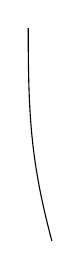
\begin{tikzpicture}\draw (0,2.7) to[out=-90,in=105] (.3,0);\end{tikzpicture}}}

Il faut prouver que l'hom
\[
\Omega_{K/k}\otimes_K A\unsure{\text{---}|\longrightarrow}\Omega_{A/k}
\]
n'a pas d'inverse à gauche, i.e. qu'il
n'existe pas de dérivation
\[
D:A\unsure{\text{---}|\longrightarrow}\Omega_{K/k}\otimes_K A
\]
qui sur $K$ induise $d_{K/k}\otimes_K\unsure{1_A}$. Or
si on avait une telle $D$, alors les
$D(t_i)$ \unsure{seront|seraient} dans un sous-module
$V\otimes_K A$, $V\subset\Omega_{K/k}$ de dim finie, donc
il existerait une \unsure{coextension|extension} de \uline{type fini}
$k'$ de $k$, telle que les $Dt_i$ soient dans
$\operatorname{Im}\Omega_{k'/k}\otimes_{k'}A$, donc leurs images dans
$\Omega_{K/k'}\otimes_K A$ \unsure{seront|seraient} nulles. \unsure{Donc quitte}
à remplacer $k$ par $k'$, [ce qui
ne change pas \unsure{l'hyp. !}] on peut supposer

\deleted{M. DUFOUR\\
VARITYPISTE\\
131, RUE LECOURBE\\
PARIS XV$^{\mathrm e}$\\
\figure{\begin{tikzpicture}\fill (0,0) rectangle (.12,.12);\end{tikzpicture}}\\
C. C. P. Paris 14.143-34\\
R. M. 140.029}
\figure{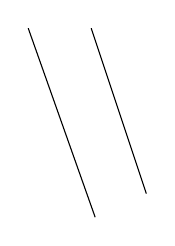
\begin{tikzpicture}\draw (0,2.4)--(.85,0);\draw (.8,2.4)--(1.5,.3);\end{tikzpicture}}

\mspage{23}
